\begin{frame}
	\myheading{Module 2.7: Linearly Separable Boolean Functions}
\end{frame}


\begin{frame}
	\begin{itemize}\justifying
		\item<1-> So what do we do about functions which are not linearly separable ?
		\item<2-> Let us see one such simple boolean function first ?
	\end{itemize}
\end{frame}


\begin{frame}
	\begin{columns}
		\column{0.6\textwidth}
		\begin{overlayarea}{\textwidth}{\textheight}
			\begin{center}
				\begin{table}
					\begin{tabular}{cccc}
						\hline
						$x_1$ & $x_2$ & XOR  \\\hline
						$0$ & $0$ & 0 & $w_0 + \sum_{i=1}^{2} w_i x_i < 0$    \\
						$1$ & $0$ & 1 & $w_0 + \sum_{i=1}^{2} w_i x_i \geq 0$ \\
						$0$ & $1$ & 1 & $w_0 + \sum_{i=1}^{2} w_i x_i \geq 0$ \\
						$1$ & $1$ & 0 & $w_0 + \sum_{i=1}^{2} w_i x_i < 0$    \\
						\hline
					\end{tabular}
				\end{table}
				\begin{align*}
					\onslide<2->{w_0 + w_1\cdot0 + w_2\cdot0 < 0    & \implies w_0 < 0}          \\
					\onslide<3->{w_0 + w_1\cdot0 + w_2\cdot1 \geq 0 & \implies w_2 > -w_0}       \\
					\onslide<4->{w_0 + w_1\cdot1 + w_2\cdot0 \geq 0 & \implies w_1 > -w_0}       \\
					\onslide<5->{w_0 + w_1\cdot1 + w_2\cdot1 \geq 0 & \implies w_1 + w_2 < -w_0}
				\end{align*}
			\end{center}
			\begin{itemize}\justifying
				\item<6-> The fourth condition contradicts conditions 2 and 3
				\item<7-> Hence we cannot have a solution to this set of inequalities
			\end{itemize}
		\end{overlayarea}
		\column{0.4\textwidth}
		\begin{overlayarea}{\textwidth}{\textheight}
			\onslide<7->{
				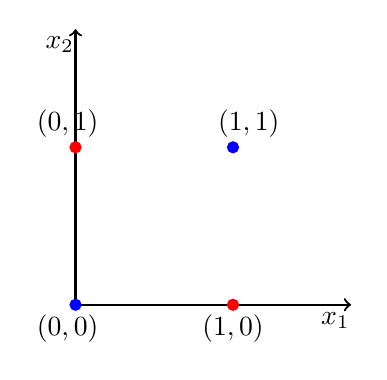
\begin{tikzpicture}
	\draw[thick,->] (0,0) -- (3.5,0);
	\draw[thick,->] (0,0) -- (0,3.5);

	\node at (3.3, -0.2) {$x_1$};
	\node at (-0.2, 3.3) {$x_2$};

	\node at (-0.1, -0.3) {$(0,0)$};
	\node at (-0.1, 2.3) {$(0,1)$};
	\node at (2.0, -0.3) {$(1,0)$};
	\node at (2.2, 2.3) {$(1,1)$};

	\filldraw[blue] (0,0) circle (2pt);
	\filldraw[red] (0,2) circle (2pt);
	\filldraw[red] (2,0) circle (2pt);
	\filldraw[blue] (2,2) circle (2pt);
\end{tikzpicture}
			}
			\begin{itemize}\justifying
				\item<8-> And indeed you can see that it is impossible to draw a line which separates the red points from the blue points
			\end{itemize}
		\end{overlayarea}
	\end{columns}
\end{frame}

\begin{frame}
	\begin{columns}
		\column{0.4\textwidth}
		\begin{overlayarea}{\textwidth}{\textheight}
						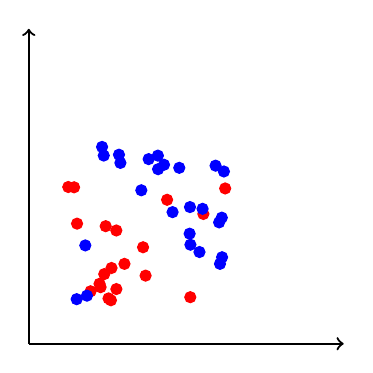
\begin{tikzpicture}
				\filldraw[red] (1.717248,1.148263) circle (2pt);
				\filldraw[blue] (1.022337,1.844630) circle (2pt);
				\filldraw[blue] (0.929218,1.449012) circle (2pt);
				\filldraw[red] (1.256599,1.328157) circle (2pt);
				\filldraw[blue] (1.917421,1.041134) circle (2pt);
				\filldraw[blue] (1.552910,0.757361) circle (2pt);
				\filldraw[red] (0.476688,0.993158) circle (2pt);
				\filldraw[blue] (1.139669,1.889055) circle (2pt);
				\filldraw[red] (1.994183,1.472244) circle (2pt);
				\filldraw[red] (0.611827,0.938297) circle (2pt);
				\filldraw[blue] (1.954791,0.598560) circle (2pt);
				\filldraw[red] (0.113127,1.025315) circle (2pt);
				\filldraw[blue] (1.547272,1.235639) circle (2pt);
				\filldraw[blue] (1.667688,0.664851) circle (2pt);
				\filldraw[blue] (0.108270,0.066074) circle (2pt);
				\filldraw[red] (1.551238,0.091185) circle (2pt);
				\filldraw[red] (0.550644,0.461861) circle (2pt);
				\filldraw[blue] (1.326191,1.171462) circle (2pt);
				\filldraw[red] (0.285269,0.166320) circle (2pt);
				\filldraw[blue] (0.645487,1.900755) circle (2pt);
				\filldraw[red] (0.715271,0.514446) circle (2pt);
				\filldraw[blue] (0.239037,0.110620) circle (2pt);
				\filldraw[blue] (1.707163,1.213513) circle (2pt);
				\filldraw[blue] (0.663682,1.796715) circle (2pt);
				\filldraw[red] (0.512817,0.075660) circle (2pt);
				\filldraw[blue] (1.542905,0.897760) circle (2pt);
				\filldraw[blue] (1.928409,0.514645) circle (2pt);
				\filldraw[blue] (0.430763,1.999726) circle (2pt);
				\filldraw[red] (0.411993,0.218422) circle (2pt);
				\filldraw[red] (0.951387,0.725352) circle (2pt);
				\filldraw[red] (0.001601,1.490619) circle (2pt);
				\filldraw[red] (0.983530,0.364934) circle (2pt);
				\filldraw[red] (0.612532,0.194346) circle (2pt);
				\filldraw[blue] (1.217355,1.773029) circle (2pt);
				\filldraw[red] (0.398657,0.261244) circle (2pt);
				\filldraw[blue] (0.452156,1.890002) circle (2pt);
				\filldraw[red] (0.458527,0.384611) circle (2pt);
				\filldraw[blue] (1.977895,1.687690) circle (2pt);
				\filldraw[blue] (0.217980,0.748811) circle (2pt);
				\filldraw[red] (0.075486,1.486788) circle (2pt);
				\filldraw[blue] (1.872187,1.761516) circle (2pt);
				\filldraw[blue] (1.142016,1.716686) circle (2pt);
				\filldraw[blue] (1.411278,1.734101) circle (2pt);
				\filldraw[blue] (1.951329,1.101424) circle (2pt);
				\filldraw[red] (0.543241,0.052208) circle (2pt);

				\draw[thick,->] (-0.5,-0.5) -- (3.5,-0.5);
				\draw[thick,->] (-0.5,-0.5) -- (-0.5,3.5);


			\end{tikzpicture}
			\only<3->{
				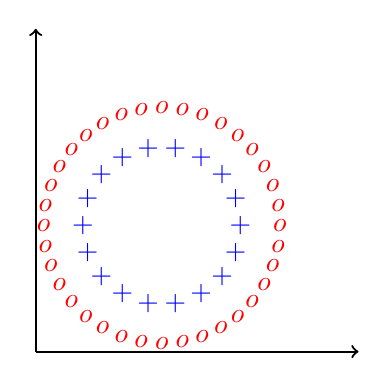
\begin{tikzpicture}
	\foreach \a in {1,2,...,18}{
			\draw (\a*360/18: 1cm) node{\color{blue}{$+$}};
		}
	\foreach \a in {1,2,...,36}{
			\draw (\a*360/36: 1.5cm) node{\color{red}{$o$}};
		}

	\draw[thick,->] (-1.6,-1.6) -- (2.5,-1.6);
	\draw[thick,->] (-1.6,-1.6) -- (-1.6,2.5);

\end{tikzpicture}
			}
		\end{overlayarea}
		\column{0.6\textwidth}
		\begin{overlayarea}{\textwidth}{\textheight}
			\begin{itemize}\justifying
				\item<1-> Most real world data is not linearly separable and will always contain some outliers
				\item<2-> In fact, sometimes there may not be any outliers but still the data may not be linearly separable
				\item<3-> We need computational units (models) which can deal with such data
				\item<4-> While a single perceptron cannot deal with such data, we will show that a network of perceptrons can indeed deal with such data
			\end{itemize}
		\end{overlayarea}
	\end{columns}
\end{frame}


\begin{frame}
	\begin{itemize}\justifying
		\item<1-> Before seeing how a network of perceptrons can deal with linearly inseparable data, we will discuss boolean functions in some more detail ...
	\end{itemize}
\end{frame}


\begin{frame}
	\begin{itemize}\justifying
		\item How many boolean functions can you design from 2 inputs ?
		\item<2-> Let us begin with some easy ones which you already know ..
		      \onslide<3->{
		      	  \footnotesize{
			      \begin{table}
				      \begin{tabular}{cccccccccccccccccc}
					      \hline

					      \onslide<3->{$x_1$} & \onslide<3->{$x_2$} & \onslide<4->{$f_1$} & \onslide<6->{$f_2$} & \onslide<8->{$f_3$} & \onslide<9->{$f_4$} & \onslide<10->{$f_5$} & \onslide<11->{$f_6$} & \onslide<12->{$f_7$} & \onslide<7->{$f_8$} & \onslide<13->{$f_9$} & \onslide<14->{$f_{10}$} & \onslide<15->{$f_{11}$} & \onslide<16->{$f_{12}$} & \onslide<17->{$f_{13}$} & \onslide<18->{$f_{14}$} & \onslide<19->{$f_{15}$} & \onslide<5->{$f_{16}$} \\
					      \hline
					      \onslide<3->{0}     & \onslide<3->{0}     & \onslide<4->{0}     & \onslide<6->{0}     & \onslide<8->{0}     & \onslide<9->{0}     & \onslide<10->{0}     & \onslide<11->{0}     & \onslide<12->{0}     & \onslide<7->{0}     & \onslide<13->{1}     & \onslide<14->{1}        & \onslide<15->{1}        & \onslide<16->{1}        & \onslide<17->{1}        & \onslide<18->{1}        & \onslide<19->{1}        & \onslide<5->{1}        \\
					      \onslide<3->{0}     & \onslide<3->{1}     & \onslide<4->{0}     & \onslide<6->{0}     & \onslide<8->{0}     & \onslide<9->{0}     & \onslide<10->{1}     & \onslide<11->{1}     & \onslide<12->{1}     & \onslide<7->{1}     & \onslide<13->{0}     & \onslide<14->{0}        & \onslide<15->{0}        & \onslide<16->{0}        & \onslide<17->{1}        & \onslide<18->{1}        & \onslide<19->{1}        & \onslide<5->{1}        \\
					      \onslide<3->{1}     & \onslide<3->{0}     & \onslide<4->{0}     & \onslide<6->{0}     & \onslide<8->{1}     & \onslide<9->{1}     & \onslide<10->{0}     & \onslide<11->{0}     & \onslide<12->{1}     & \onslide<7->{1}     & \onslide<13->{0}     & \onslide<14->{0}        & \onslide<15->{1}        & \onslide<16->{1}        & \onslide<17->{0}        & \onslide<18->{0}        & \onslide<19->{1}        & \onslide<5->{1}        \\
					      \onslide<3->{1}     & \onslide<3->{1}     & \onslide<4->{0}     & \onslide<6->{1}     & \onslide<8->{0}     & \onslide<9->{1}     & \onslide<10->{0}     & \onslide<11->{1}     & \onslide<12->{0}     & \onslide<7->{1}     & \onslide<13->{0}     & \onslide<14->{1}        & \onslide<15->{0}        & \onslide<16->{1}        & \onslide<17->{0}        & \onslide<18->{1}        & \onslide<19->{0}        & \onslide<5->{1}        \\
					      \hline
				      \end{tabular}
			      \end{table}}
		      }
		\item<20-> Of these, how many are linearly separable ? \onslide<21->{(turns out all except XOR and !XOR - feel free to verify)}
		\item<22-> In general, how many boolean functions can you have for $n$ inputs ? \onslide<23->{$2^{2^n}$}
		\item<24-> How many of these $2^{2^n}$ functions are not linearly separable ? \onslide<25->{For the time being, it suffices to know that at least some of these may not be linearly inseparable (I encourage you to figure out the exact answer :-) )}
	\end{itemize}
\end{frame}

